\documentclass[12pt]{article}
\usepackage{amsmath}
\usepackage{amssymb}
%\usepackage{hyperref}
\usepackage{epsfig,graphicx,amsmath}
\usepackage{amsfonts}
\usepackage{enumerate}
\usepackage{amsfonts}
\usepackage{amssymb}
\usepackage{amsthm}


\newcommand{\mb}[1]{\mbox{\boldmath$#1$}}
\newcommand{\p}{\partial}
\newcommand{\ds}{\displaystyle}
\newcommand{\beq}{\begin{eqnarray}}
\newcommand{\beqq}{\begin{eqnarray*}}
\newcommand{\eeq}{\end{eqnarray}}
\newcommand{\eeqq}{\end{eqnarray*}}
\newcommand{\eps}{\varepsilon}
\newcommand{\erf}{\mbox{erf}}
\newcommand{\erfi}{\mbox{erfi}}
\newcommand{\Ei}{\mbox{Ei}}
\newcommand{\x}{\mbox{\boldmath$x$}}
\newcommand{\Aa}{\mbox{\boldmath$A$}}
\newcommand{\rr}{\mbox{\boldmath$r$}}
\newcommand{\As}{\mbox{\boldmath$a$}}
\newcommand{\y}{\mbox{\boldmath$y$}}
\newcommand{\z}{\mbox{\boldmath$z$}}
\newcommand{\J}{\mbox{\boldmath$J$}}
\newcommand{\ET}{\mbox{\boldmath$\eta$}}
\newcommand{\n}{\mbox{\boldmath$n$}}
\newcommand{\X}{\mbox{\boldmath$X$}}
\newcommand{\Y}{\mbox{\boldmath$Y$}}
\newcommand{\Yy}{\mbox{\boldmath$y$}}
\newcommand{\Z}{\mbox{\boldmath$Z$}}
\newcommand{\w}{\mbox{\boldmath$w$}}
\newcommand{\vv}{\mbox{\boldmath$v$}}
\newcommand{\bb}{\mbox{\boldmath$b$}}
\newcommand{\Bb}{\mbox{\boldmath$b$}}
\newcommand{\B}{\mbox{\boldmath$B$}}
\newcommand{\ALPHA}{\mbox{\boldmath$\alpha$}}
\newcommand{\aaa}{\mbox{\boldmath$a$}}
\newcommand{\C}{\mbox{\boldmath$C$}}
\newcommand{\SSigma}{\mbox{\boldmath$\Sigma$}}
\newcommand{\mmu}{\mbox{\boldmath$\mu$}}
\newcommand{\IIm}{\mbox{\boldmath$I_m$}}
\newcommand{\mean}[1]{\langle #1\rangle}
\newcommand{\diffunit}{$\mu$m$^2$.s$^{-1}$}
\newcommand{\Li}{\mbox{Li}}
\newcommand{\thet}{\mbox{\boldmath$\theta$}}
\newcommand{\intR}{\int\limits_{\mathbb{R}}}
\newcommand{\intRm}{\int\limits_{\mathbb{R}^m}}
\newcommand\norm[1]{\left\lVert#1\right\rVert}
%\definecolor{red}{rgb}{1,0,0}

\usepackage{color}
\usepackage{float}
\begin{document}	
	\title{Results \& Material and methods}
	\author{Ofir Shukron \& David Holcman}
	\maketitle
	
	\section{Result section}
	To estimate the nucleosome reorganization following DNA damages, we have
	constructed a mathematical model, where redistribution can be due either to chromatin de-
	compaction or nucleosome sliding along the chromatin or both of them. We
	have used the model to assess the relative contribution of these two processes
	to the total DNA and nucleosome signal loss from a region of interest (ROI),
	a quantity which is inaccessible experimentally.
	
	The model (presented in Material and methods) follows the DNA, $D(u)$,
	and nucleosome, $H(u)$, fraction of signal loss from the ROI as a function of
	the UV dose, $u$. We have used the measured H3.3 and DNA signal loss to
	calibrate parameters of nucleosome and DNA models respectively (Fig. 3A-
	D). Using the calibrated models we have found that the relative contribution
	of nucleosome sliding to the total signal loss in the ROI is monotonically
	decreasing from 75\% to 70\% for nucleosomes and 51\% to 40\% for DNA loss,
	as the UV dose increases from 5 to 100 msec. The remaining percentages are
	attributed to chromatin expansion and de-compaction (see Figure \ref{fig:relatiiveContributionToLoss}).
	
	\begin{figure}[H]
		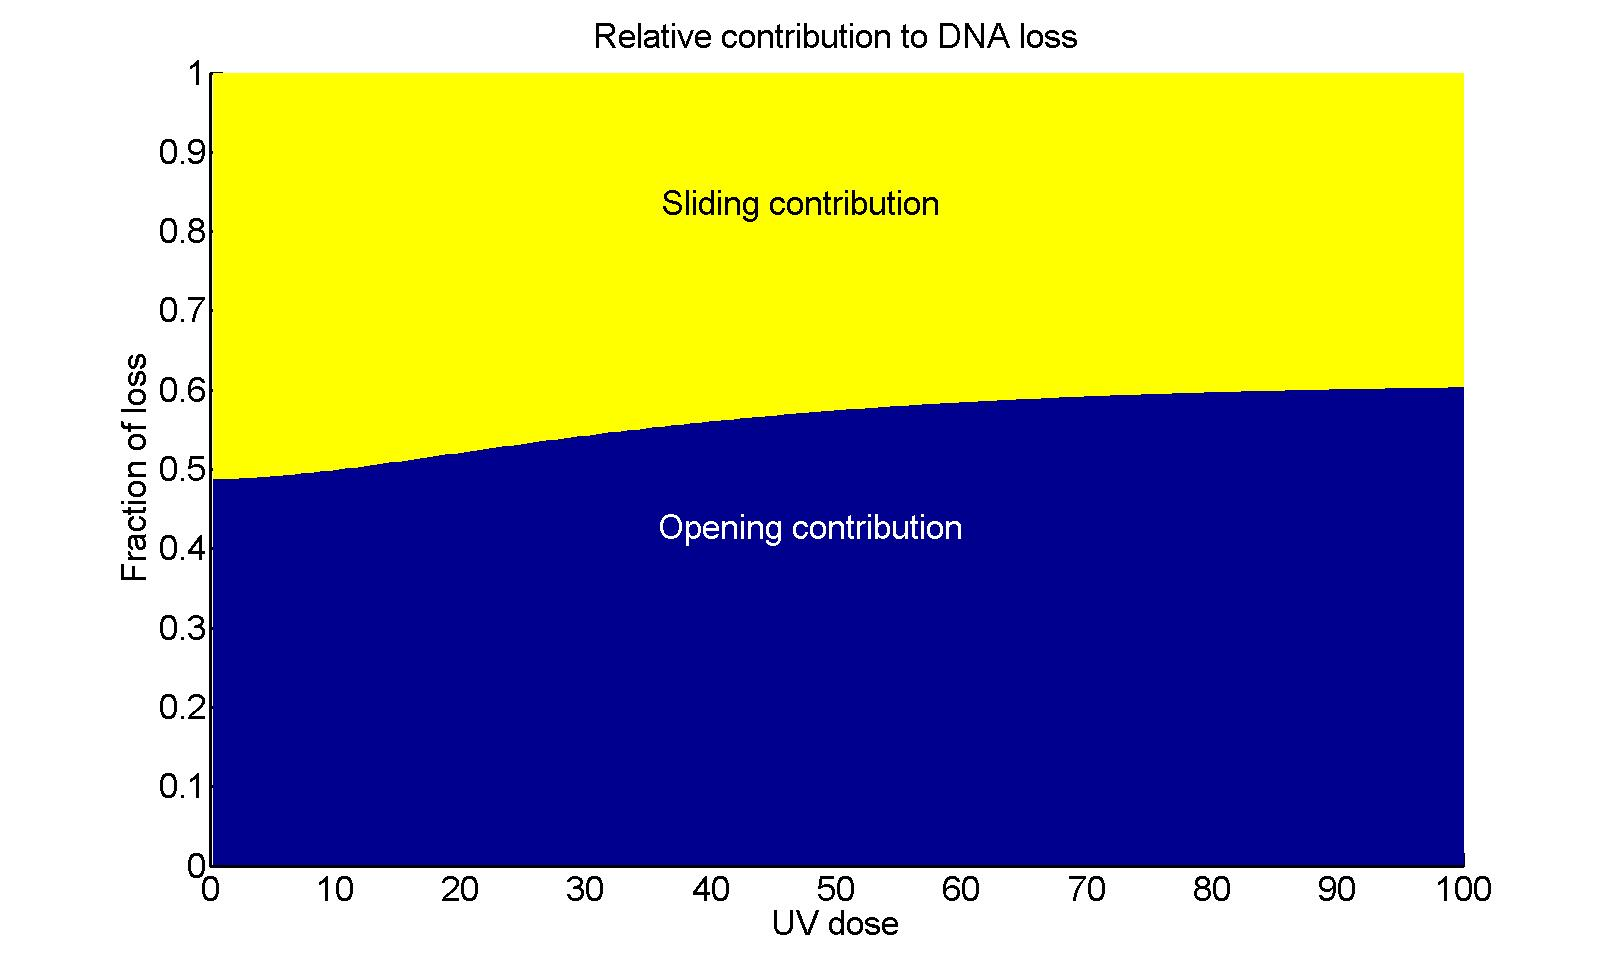
\includegraphics[width=0.5\linewidth, height=0.3\textheight]{relatiiveContributionToDNALoss}
		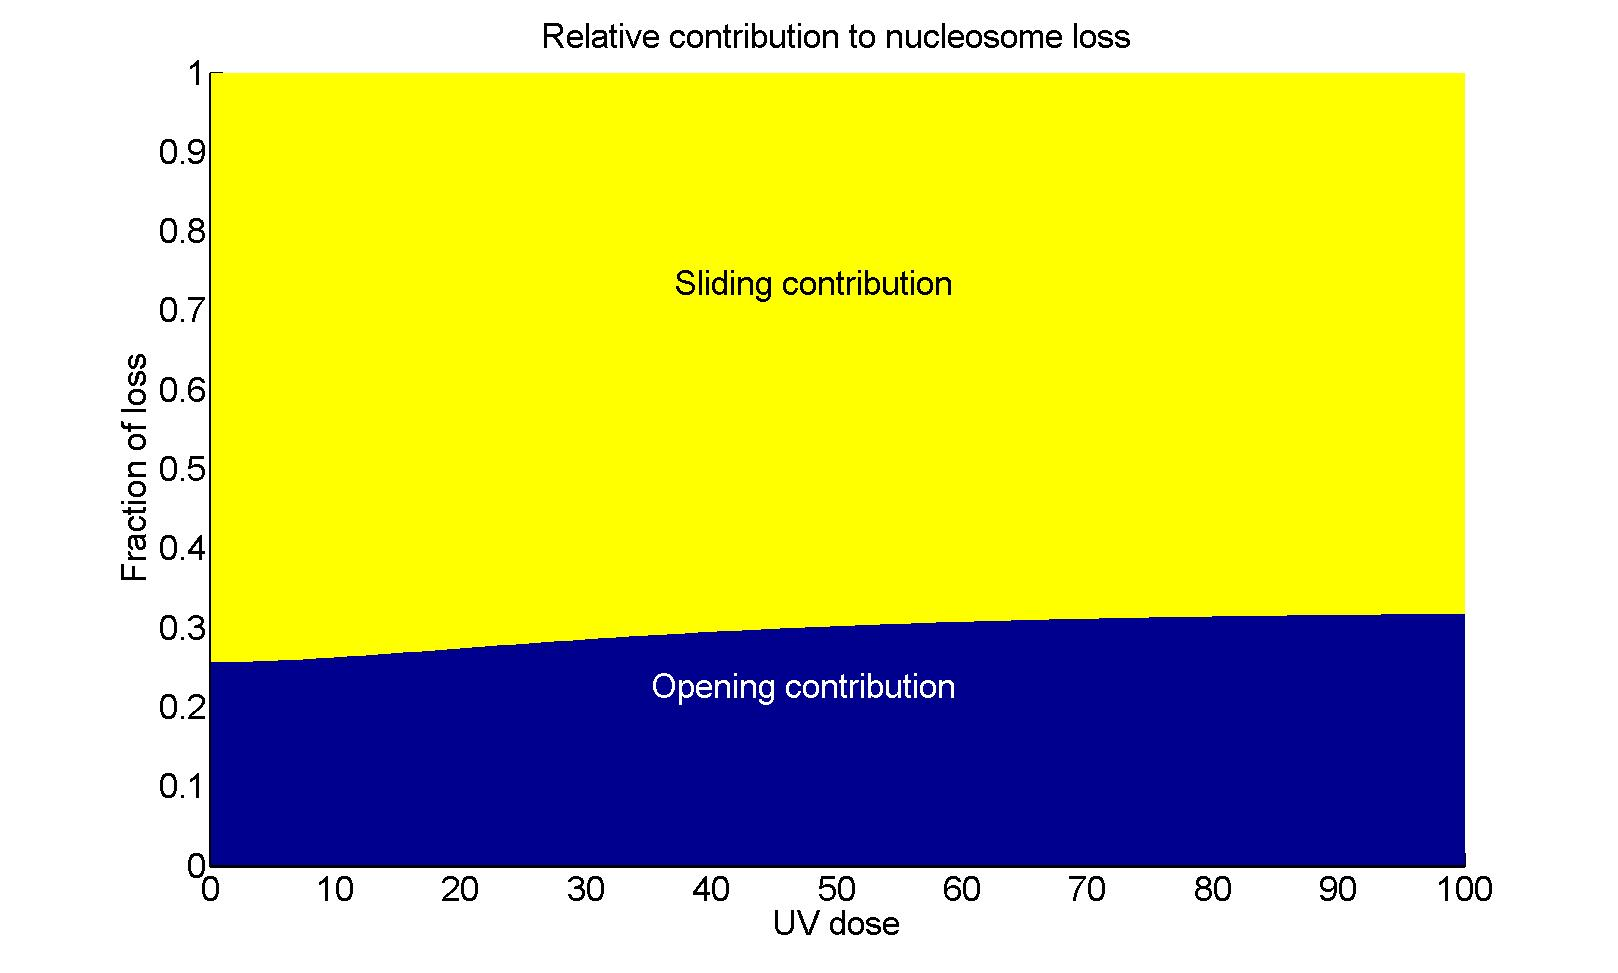
\includegraphics[width=0.5\linewidth, height=0.3\textheight]{relativeContributionToHistoneLoss}
		\caption{\textbf{Relative contribution of chromatin opening and nucleosome sliding to DNA (left) and histone (right) loss}. Sliding contribution is monotonically decreasing with UV dose for both DNA and nucleosome signals. The increase in chromatin opening contribution is due to the increase in chromatin reorganization following high dosages of UV, which is responsible for the majority of signal loss.}
		\label{fig:relatiiveContributionToLoss}
	\end{figure}
	
 \section{Material and methods: Modeling nucleosomes and DNA redistribution following UV damages} 
	
	We present here a model for nucleosomes and DNA re-organization following
	UV damages. The cascade of events leading to tagged DNA and nucleosomes'
	redistribution, results in signal extrusion from a region of interest (ROI) up
	to a maximal loss, measured 15 minutes post UV-C.
	
	\subsection{Dynamics of nucleosomes following UV damages in the region of interest}
	
	Following the experimental protocol, a two-dimensional circular initial damage region (IDR), induced by the UV-C laser, is centered around the focal point (origin of the coordinates) with a fixed area of $A_0$. Following
	laser induction with a UV dose $u$ $[msec]$, the damaged region expands radially outward and reaches its maximal area of $A(u)$ after 15 minutes. At the end of expansion, the circular region is defined	as the ROI, in which DNA and nucleosome signals are measured at
	time 0 and 15 minutes. The fraction of signal loss is calculated for DNA and nucleosomes as
	\begin{equation*}
	\frac{signal(0)-signal(15)}{signal(0)}
	\end{equation*}	
	where $signal(0)$ and $signal(15)$ are the DNA or nucleosome signals at time 0 and 15 minutes respectively. 
	
	We assume that the loss of DNA and nucleosome signals post UV-C is due
	to two mechanisms: the first is chromatin expansion, and the second is nucleosomes sliding along the chromatin. For chromatin expansion, recruitment of repair and chromatin remodeling factors to bind to damaged DNA causes chromatin de-compaction and cross-links break \cite{luijsterburg2012ddb2} to enable repair factor access to damages \cite{gaillard2003chromatin}. Because the majority of damages are inflicted around the laser's focal point, the accumulation of repair factors there \cite{dinant2007activation} will generate a pushing force on chromatin outside the DR in a radial outward direction. As a result, DNA and nucleosome outside the DR will be extruded from the ROI in equal proportions. 
	
	An additional proportion of nucleosome signal loss is caused by the mechanism of nucleosome sliding. Repair proteins slide nucleosomes wrapped by damaged DNA away from high concentration of DNA damages (see Figure NNN) to facilitate efficient repair \cite{gaillard2003chromatin}. Sliding nucleosomes out of the DR loosens the chromatin in the DR and exposes damaged DNA. Remodeling and repair proteins, binding to the exposed damaged position, further contribute to the pushing of undamaged DNA outside the DR while retaining damaged DNA within it.  

    In-line with the description above, we construct a model representing
	signal loss 15 minutes post UV-C. We do not specifically take into account the
	mechanism of signal loss in time and only present equations representing the maximal loss of signal as a function of the UV dose.
	
	\subsection{Dynamics of DNA and nucleosome loss from the DR}
	The IDR and the ROI are considered to be two-dimensional concentric circular regions, characterized by an area $A_0$ and $A(u)$, respectively. We assume an initial uniform distribution of DNA in the IDR and its vicinity, such that the amount of DNA in $A(u)$ is $c_dA(u)$, with $c_d$ in units of $bp/\mu m^2$. 
	
	We restrict DNA damages to be inflicted in $A_0$ immediately after UV induction. We set $T(u)$ to represent the amount of damaged DNA left in $A(u)$ 15 minutes post UV-C, while the undamaged DNA is assumed to be extruded. Therefore, the fraction of DNA signal loss, $D(u)$, is calculated as the ratio of the extruded DNA to the total amount of DNA in the ROI, $c_dA(u)$. 
	\begin{equation}\label{eq:DNALossFraction}
	D(u) = \frac{c_dA(u)- T(u)}{c_dA(u)}
	\end{equation}
	
	Similarly to the DNA, we assume that the number of nucleosome in a $A(u)$ is $c_nA(u)$, with $c_n$ a constant in units of $nucleosomes/\mu m^2$. The total fraction of nucleosome extruded from the ROI, $H(u)$, is calculated as the sum of nucleosomes pushed with undamaged DNA and the ones sliding out.
	\begin{equation}\label{eq:nucleosomeLossFraction}
	H(u) = D(u) + \frac{N_S(u)}{c_nA(u)}	
	\end{equation}
	
	In order to evaluate the fractions in \eqref{eq:DNALossFraction} and \eqref{eq:nucleosomeLossFraction}, we shall first formulate a model for the damaged DNA in the DR, $T(u)$ and derive $A(u)$ and $N(u)$ based on it.
	
	\subsection{DNA damages in the IDR as a function of the UV dose}\label{subsection:AccumulationOfDNADamagesInTheIDR}
	We assume that the rate of accumulation of DNA damages in the
	$A_0(u)$ with increasing UV dose is proportional to the undamaged DNA in $A_0(u)$ [REF]. Therefore,	
	\begin{equation}\label{eq:DNADamageRate}
	\frac{dT(u)}{du} = k_t(c_dA_0(u) - T(u))
	\end{equation}	
	with $k_t$ a constant. Using the initial condition $T(0) = 0$, the solution to equation \eqref{eq:DNADamageRate} is
	\begin{equation}\label{eq:DNADamagedIDR}
	T(u) = c_dA_0(1-\exp(-k_tu))
	\end{equation}
	
	\subsection{Deriving the functions describing loss of nucleosome from the IDR and the ROI expansion}
	We now turn to construct a model for the number of nucleosomes $N(u)$
	extruded from the DR and subsequently out of the ROI as a function of the UV dose. Although the exact mechanism by which nucleosome are lost is not known, we will describe the loss by that contribution of chromatin expansion and nucleosome sliding out of the DR. Hence,
	\begin{equation}\label{eq:nucleosomesAsSumDR}
	N(u)=N_P(u)+N_S(u)
	\end{equation}
	where $N_P(u)$ is the number of nucleosomes pushed with undamaged DNA and $N_S(u)$ is the number of nucleosomes sliding out of the DR.
	
	According to our assumption, the undamaged DNA is pushed out of the DR, therefore we can write
	\begin{equation}\label{eq:nucleosomePushDR}
	N_P(u) = k_pT(u)
	\end{equation}	
	with $k_p$ a constant of units $nucleosomes/bp $. 
	
	We propose that the rate of nucleosomes leaving the DR by sliding is proportional to the fraction of nucleosomes affected by increase of UV dose in $A_0$. In the first-order approximation, the dynamics of nucleosomes sliding, $N_S(u)$, is given by
	\begin{equation}\label{eq:nucleosomeSlideRate}
	\frac{dN_S(u)}{du} = k_s\left( c_nA_0-N(u))\right)\frac{dT(u)}{du}	
	\end{equation}
	with $k_s$ a constant of units $1/bp$. 
	
	We note that differentiating equation \eqref{eq:nucleosomesAsSumDR} with respect to $u$ leads to 
	\begin{equation}
	\frac{dN(u)}{du}=\frac{dN_P(u)}{du} +\frac{dN_S(u)}{du}
	\end{equation}	
	Therefore, differentiating equation \eqref{eq:nucleosomePushDR} and adding to it \eqref{eq:nucleosomeSlideRate} we obtain the rate equation for $N(u)$ 
	\begin{equation}\label{eq:nucleosomeRateDR}
	\frac{dN(u)}{du}= \left(k_s(c_nA_0-N(u))-k_p\right)\frac{dT(u)}{du}
	\end{equation}
	 Using the initial condition $N(0) = 0$, the solution of equation \eqref{eq:nucleosomeRateDR} is 
	 
	\begin{equation}\label{eq:nucleosomeLossDR}
	N(u) = \left(c_nA_0-\frac{k_p}{k_s}\right)\left(1-\exp\left(-k_sT(u)\right)\right)
	\end{equation}	
	and the number of nucleosomes sliding out of the DR is 
	\begin{equation}\label{eq:nucleosomeSlideDR}
	N_S(u) = N(u)-N_P(u)
	\end{equation}
	Next, we model the dynamics of the ROI area $A(u)$ with increasing UV
	dose. For this end, we consider a linear increase of ROI radius, $R(u)$, with sliding and chromatin de-compaction (see Figure NNN). 
		
	\begin{equation*}
	\frac{dR(u)}{du}=k_a\left(\frac{dN_P(u)}{du}+\frac{dN_S(u)}{du}\right)= k_a\frac{dN(u)}{du}
	\end{equation*}
	where $k_a$ is a constant of units $\mu m/ nucleosomes$. Using the initial condition $R(0) = R_0$, we find
	\begin{equation}
	R(u) = R_0+ k_aN(u)
	\end{equation}
	The ROI area is then 
	\begin{equation}\label{eq:ROIarea}
	A(u)= \pi R(u)^2 = \pi (R_0+k_aN(u))^2
	\end{equation}
	where we consider $R_0$ to represent the radius of the IDR even in the absence of UV induction.
	
	We can now substitute the functions \eqref{eq:DNADamagedIDR}, \eqref{eq:nucleosomeSlideDR}, \eqref{eq:ROIarea} into the equations \eqref{eq:DNALossFraction} and \eqref{eq:nucleosomeLossFraction} to get the expressions for $D(u)$ and $H(u)$. We present the functions in terms of $T(u)$
	\begin{equation}\label{eq:DNALoss}
	D(u) = \frac{\frac{N(u)}{N_0}\left(\frac{k_p(1-k_s)}{k_p(1-k_s)+k_s}-\frac{k_aN_0}{A_0}\right)+\frac{k_aN_0}{A_0}}{1+\frac{k_aN_0}{A_0}\left(1-\frac{N_T(u)}{N_0}\right)}
	\end{equation}
	\begin{equation}\label{eq:nucleosomeLoss}
		H(u) = \frac{\frac{N_T(u)}{N_0}\left(1-\frac{k_aN_0}{A_0}\right)+\frac{k_aN_0}{A_0}}{1+\frac{k_aN_0}{A_0}\left(1-\frac{N_T(u)}{N_0}\right)}
	\end{equation}
	
	\subsection{Parameter fit for $D(u)$ and $H(u)$}\label{subsection:parameterFit}
	We now use equations \eqref{eq:DNALoss}  and \eqref{eq:nucleosomeLoss} to fit the experimental data. We simultaneously fit equations \eqref{eq:DNALoss}  and \eqref{eq:nucleosomeLoss} to the H3.3 and DNA loss data, with the goal of maximizing the $R^2$ of both equations. Excluding the measurement at 5 msec, and using classical fitting procedure, we find
	\begin{equation*}
	k_t = 0.037, \quad k_s = 0.35,\quad k_p = 0.24, \quad \frac{k_aN_0}{A_0} = 0.46
	\end{equation*}
	with $R^2 = 0.93$ and $R^2 = 0.96$ for DNA and nucleosome loss fit respectively.
	
	
\begin{figure}[H]
\centering
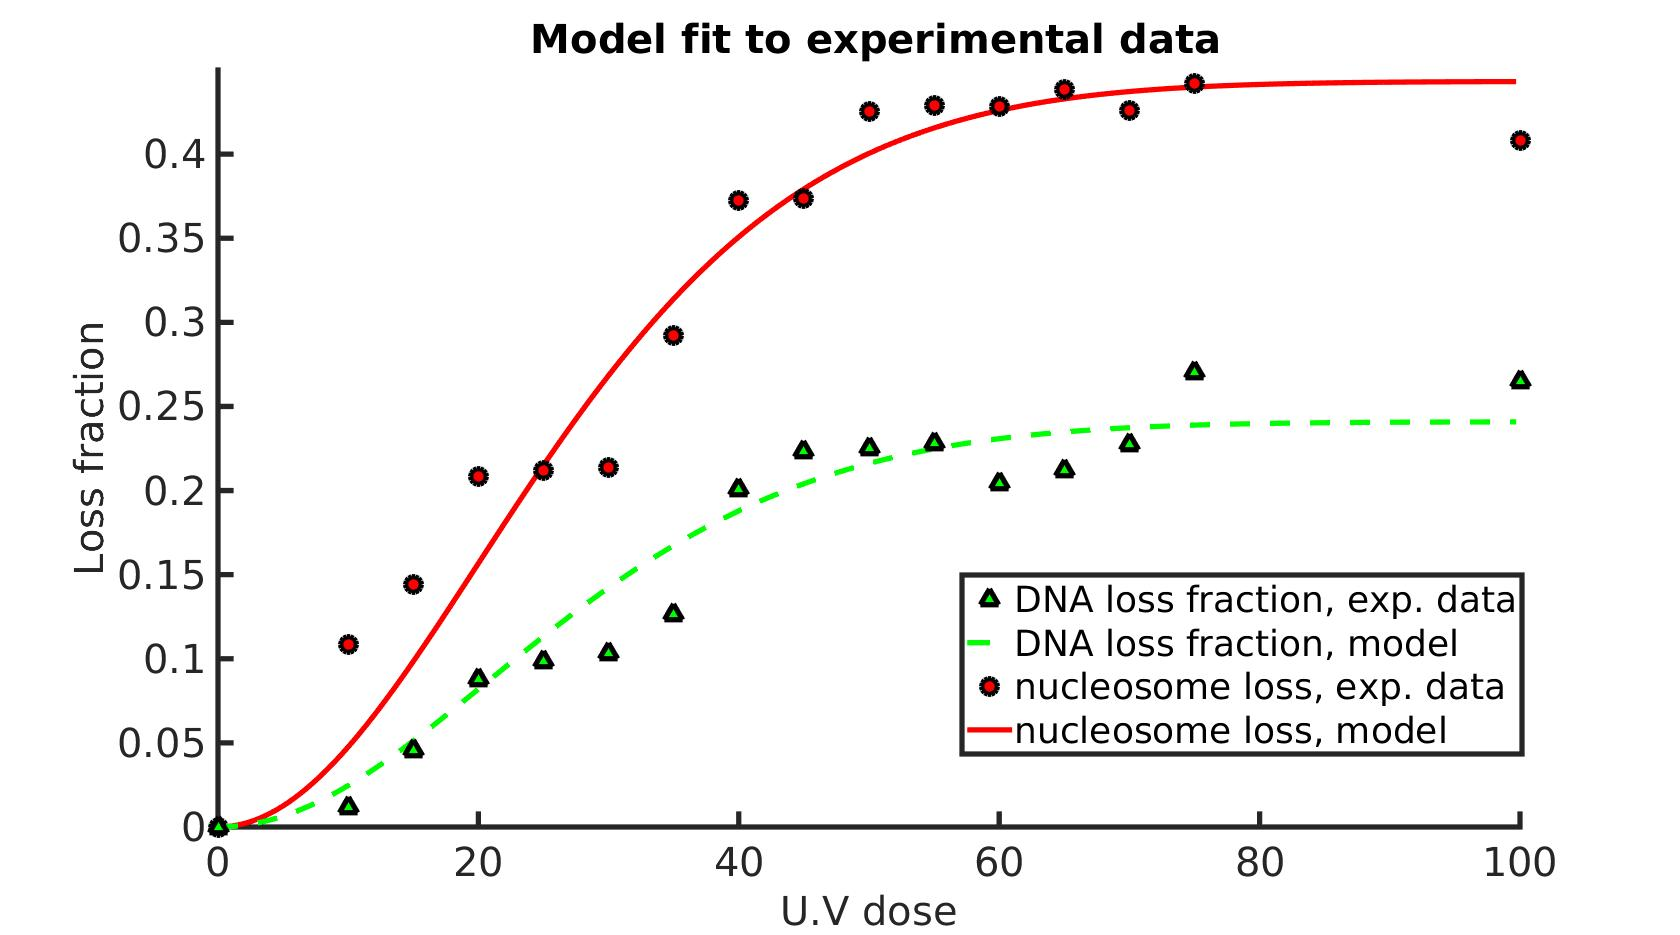
\includegraphics[width=0.5\linewidth, height=0.3\textheight]{histoneAndDnaVsUvDoseModelFit}
\caption{\textbf{Histone (red) and DNA (green) loss: experimental data
	for nucleosomes (circle) and DNA (triangles) versus model curves
	(continuous and dashed, respectively)}. Parameter values are obtained
	by simultaneously fitting equations\eqref{eq:DNALoss}  and \eqref{eq:nucleosomeLoss} to the experimental data with
	the goal of maximizing the $R^2$. The resulting curves show $R^2 = 0.96$ and
	$R^2 = 0.93$ for nucleosome and DNA loss, respectively.}
\label{fig:histoneAndDnaVsUvDoseModelFit}
\end{figure}

\subsection{Relative contribution of opening and sliding to DNA
	and nucleosome signal loss}

Using the calibrated model in equation equations \eqref{eq:DNALoss}  and \eqref{eq:nucleosomeLoss}, we now calculate the
relative contribution of chromatin opening and nucleosome sliding to the
total loss of DNA and nucleosomes. The sliding contribution refers to all loss
caused by either directly sliding nucleosome out of the DR or as the effect
nucleosome sliding has on pushing chromatin out of the DR by operations
of repair factors. Chromatin opening contribution refers to all signal loss
caused by chromatin remodeling, which causes expansion of the DR and
subsequent loss of signal from the ROI.

We start by dividing the equation describing the ROI expansion into the
two sub-mechanisms of signal loss

\begin{equation*}
A(u) = A_P(u) +A_S(u)
\end{equation*}
with $A_P(u)$ the area attributed to chromatin opening, and $A_S(u)$ to nucleosome sliding. Subtracting the sliding contribution from the ROI expansion
in equation \eqref{eq:ROIarea}, we arrive at
\begin{equation*}
A_P(u) = A_0 + k_aN_P(u)
\end{equation*}

The DNA loss attributed to chromatin opening and de-compaction is thus
\begin{equation*}
D(u)_{opening}= \frac{A_P(u)/A_0 -1 +D_P(u)/A_0}{A_P(u)/A_0}
\end{equation*}	
The fraction attributed to chromatin opening and sliding out of the total
DNA loss are given respectively by
\begin{equation}\label{eq:relativeOpeningSlidingDNA}
\frac{D(u)_{opening}}{D(u)}, \quad \frac{D(u)_{sliding}}{D(u)}=1-\frac{D(u)_{opening}}{D(u)}
\end{equation}

Similarly, the relative contribution of chromatin opening and nucleosome
sliding to the total nucleosome loss is given respectively by
\begin{equation}\label{eq:relativeOpeningSlidingNucleosomes}
\frac{H(u)_{opening}}{H(u)} = \frac{D(u)_{opening}}{H(u)},\quad \frac{H(u)_{sliding}}{H(u)}=1-\frac{H(u)_{opening}}{H(u)}
\end{equation}

where here we have used the fact that $H(u)_{opening} = D(u)_{opening}$. Graphs of
equations \eqref{eq:relativeOpeningSlidingDNA} and \eqref{eq:relativeOpeningSlidingNucleosomes}  are presented in Figure \ref{fig:relatiiveContributionToLoss}.

\subsection{Nucleosome sliding out of the IDR}
The fraction of nucleosomes lost by sliding out of the total nucleosomes in the IDR
(and eventually pushed out of the ROI) is found to be an increasing function
of the UV dose

\begin{equation*}
N_S(u) = \frac{H(u)-D(u)}{1-D(u)}
\end{equation*}

Substituting the parameter values in subsection \ref{subsection:parameterFit} and plugging \eqref{eq:DNALoss} and \eqref{eq:nucleosomeLoss} into the expression above, we obtain the results in Figure \ref{fig:fractionSlidingOutOfIDR}, where the model
in equation \eqref{eq:nucleosomeSlide} is plotted against the experimental data ($R^2 = 0.75$).

\begin{figure}
\centering
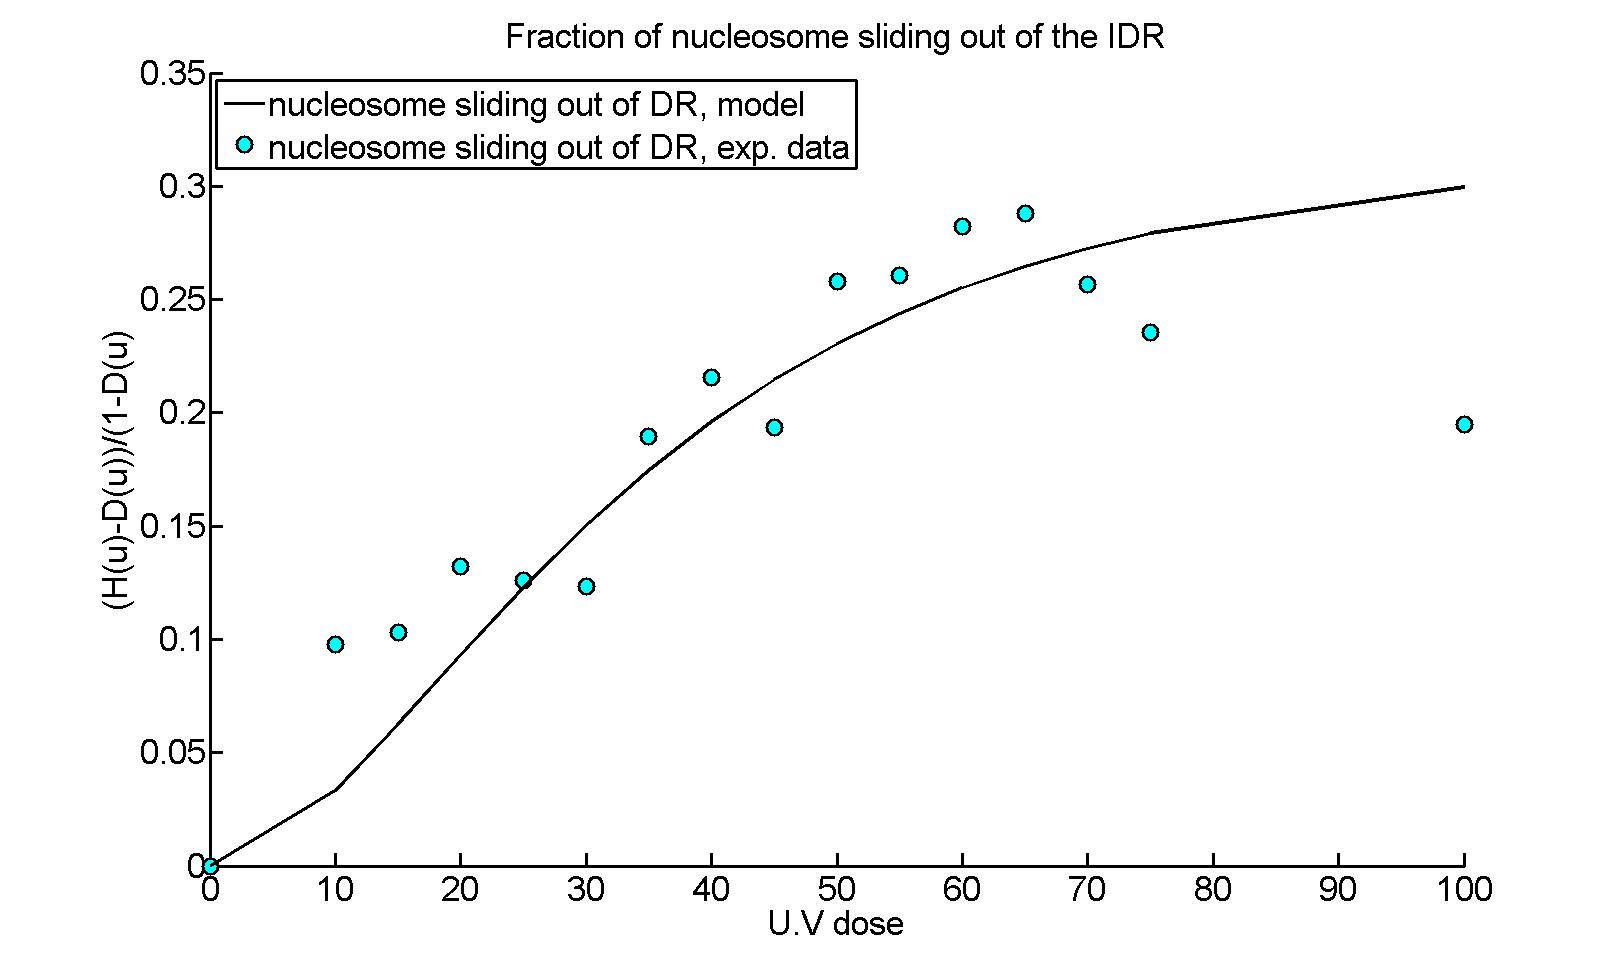
\includegraphics[width=0.5\linewidth, height=0.3\textheight]{fractionSlidingOutOfIDR}
\caption{\textbf{Fraction of nucleosomes sliding out of the IDR. The plot
		against the experimental data resulted in $R^2 = 0.75$}}
\label{fig:fractionSlidingOutOfIDR}
\end{figure}

The parameters values found in subsection \ref{subsection:parameterFit}, can further be used to estimate the fraction of nucleosome loss from the IDR attributed to sliding and
chromatin opening. These contributions are given by the leading coefficients
in the equations \eqref{eq:nucleosomePush} and \eqref{eq:nucleosomeSlide} for $N_P(u)$ and $N_S(u)$, respectively. We have, for
chromatin opening and sliding, respectively
\begin{equation*}
N_P(u) = 0.3N_T(u),\quad N_S(u) = 0.7N_T(u)
\end{equation*}

% The bibliography
\bibliographystyle{plain}
\bibliography{MaterialsAndMethodsModel.bib} % the bibliography.bib file 

\end{document}